% !TEX TS-program = pdflatex
% !TEX encoding = UTF-8 Unicode

% This is a simple template for a LaTeX document using the "article" class.
% See "book", "report", "letter" for other types of document.

\documentclass[11pt]{article} % use larger type; default would be 10pt

\usepackage[utf8]{inputenc} % set input encoding (not needed with XeLaTeX)
\usepackage[backend=biber, style=authoryear]{biblatex}
\addbibresource{bibliography.bib}
%%% Examples of Article customizations
% These packages are optional, depending whether you want the features they provide.
% See the LaTeX Companion or other references for full information.

%%% PAGE DIMENSIONS
\usepackage{geometry} % to change the page dimensions
\geometry{a4paper} % or letterpaper (US) or a5paper or....
% \geometry{margin=2in} % for example, change the margins to 2 inches all round
% \geometry{landscape} % set up the page for landscape
%   read geometry.pdf for detailed page layout information

%\usepackage{graphicx} % support the \includegraphics command and options

\usepackage[parfill]{parskip} % Activate to begin paragraphs with an empty line rather than an indent

%%% PACKAGES
\usepackage{booktabs} % for much better looking tables
\usepackage{array} % for better arrays (eg matrices) in maths
\usepackage{paralist} % very flexible & customisable lists (eg. enumerate/itemize, etc.)
\usepackage{verbatim} % adds environment for commenting out blocks of text & for better verbatim
\usepackage{subfig} % make it possible to include more than one captioned figure/table in a single float
\usepackage{graphicx}
\usepackage{multirow} % allows multipel rows per cell
% These packages are all incorporated in the memoir class to one degree or another...

%%% HEADERS & FOOTERS
\usepackage{fancyhdr} % This should be set AFTER setting up the page geometry
\pagestyle{fancy} % options: empty , plain , fancy
\renewcommand{\headrulewidth}{0pt} % customise the layout...
\lhead{}\chead{}\rhead{}
\lfoot{}\cfoot{\thepage}\rfoot{}

%%% SECTION TITLE APPEARANCE
\usepackage{sectsty}
\allsectionsfont{\sffamily\mdseries\upshape} % (See the fntguide.pdf for font help)
% (This matches ConTeXt defaults)

%%% ToC (table of contents) APPEARANCE
\usepackage[nottoc,notlof,notlot]{tocbibind} % Put the bibliography in the ToC
\usepackage[titles,subfigure]{tocloft} % Alter the style of the Table of Contents
\renewcommand{\cftsecfont}{\rmfamily\mdseries\upshape}
\renewcommand{\cftsecpagefont}{\rmfamily\mdseries\upshape} % No bold!

%%% END Article customizations

%%% The "real" document content comes below...

\title{\vspace{-3.0cm}Title}
\author{Hugh Kelley}
\date{} % Activate to display a given date or no date (if empty),
         % otherwise the current date is printed 

\begin{document}
\maketitle

\section{Abstract}

\section{List of Tables}

\section{List of Figures}

% TOC

%%%%%%%%%%%%%%%%%%%%%%%%%%%%%%%%%%%%%%%%%%%%%%%%%%%%%%%%%%%%%%%%%%%%%%%%%%%%%%%%%%%%%%%%%%%%%%%%%%%%%%%%%%%%%%%%%
\section{Research Goal and Overview}
What makes a city comfortable for cycling? The conditions are clear when one sees them, but defining the characteristics quantitatively is challenging. 

This research is intended to build a cohesive methodology for defining the overall suitability of a city to transport by bicycle. It extends the literature in three ways; extending quantitative research to a holistic approach rather than focusing on individual edges or nodes, extending holistic approaches to quantitative outcomes rather than visual or anecdotal conclusions, and by emphasizing the use of open source tools and data that are available to any member of community. 

The research provides a methodology that allows a community to identify nodes and edges for improvement that will have the largest impact on the overall network, quantify the expected improvement, and thus require from elected officials specific changes to the roads in their communities. 

\subsection{ethical risks}

This project relies entirely on publicly accessible data. 

%%%%%%%%%%%%%%%%%%%%%%%%%%%%%%%%%%%%%%%%%%%%%%%%%%%%%%%%%%%%%%%%%%%%%%%%%%%%%%%%%%%%%%%%%%%%%%%%%%%%%%%%%%%%%%%%%
\section{Introduction}


\subsection{Cycling mode share}

\subsection{The decision to cycle}

\subsection{Route Choice}

\subsection{The role of the researcher}

%%%%%%%%%%%%%%%%%%%%%%%%%%%%%%%%%%%%%%%%%%%%%%%%%%%%%%%%%%%%%%%%%%%%%%%%%%%%%%%%%%%%%%%%%%%%%%%%%%%%%%%%%%%%%%%%%
\section{Literature}

\subsection{The decision to cycle}

\subsection{Cycling Infrastructure}

\subsection{Cycling Danger}

\subsection{Cycling Networks}

\subsection{Network Analysis and Accessibility}

%%%%%%%%%%%%%%%%%%%%%%%%%%%%%%%%%%%%%%%%%%%%%%%%%%%%%%%%%%%%%%%%%%%%%%%%%%%%%%%%%%%%%%%%%%%%%%%%%%%%%%%%%%%%%%%%%
% Methods and Data need a good structure because they rely on each other
\section{Methods}

\subsection{Data Sources}

\subsubsection{Open Street Map}

Open street map provides community generated geospatial data. This data is accessible via the overpass API from several hosts. 

\subsubsection{A Close Look at an Open Street Map Case Study}

Using data from Open street map is difficult. 

Compare Relation\= cycleway to a list of edges and nodes tagged cycleway

Adding living streets and residential streets don't do much. 

Part of the problem is the lack of consistent tagging, it only takes one line segment missing a tag to disconnect two nodes,

but this also reflects the fact that getting somewhere within london nearly always requires leaving cycle infrastructure at some point and using main roads. 

The importance of this consideration will be shown using a percolation style analysis of the network, adding busier and busier roads to the network and considering the largest connected component. 

\subsubsection{2011 Census Journey to work data}

The 2011 census asked questions about where people work and how they get there. 

\subsubsection{LSOA boundaries and data}

where LSOA's were comprised of multiple polygons, the centroid of the largest polygon was used. 

lsoa population from mid 2011 
https://www.ons.gov.uk/peoplepopulationandcommunity/populationandmigration/populationestimates/datasets/lowersuperoutputareamidyearpopulationestimates

LSOA boundaries are available from the London Data store

https://data.london.gov.uk/dataset/statistical-gis-boundary-files-london

On maps created using these boundaries the copyright must be stated. This is: "Contains National Statistics data %© Crown copyright and database right [2015]" and "Contains Ordnance Survey data © Crown copyright and database right [2015]"

\subsubsection{Road KSI data}

https://www.gov.uk/government/collections/road-accidents-and-safety-statistics

https://data.london.gov.uk/dataset/pedal-cyclist-casualties-killed-and-seriously-injured

https://data.london.gov.uk/dataset/road-casualties-severity-borough

\subsection{Data import, storage, cleaning, and joining}

remove multipolygon lsoa interior rings in favor of polygon lsoa shapes

\subsection{Defining Cycle Networks}

How were the representative networks built? 

\subsection{Travel Times}

\subsection{Street Type and Street Danger}

\subsection{Accessibility}

\subsection{assumptions and concerns}

used centroids instead of actual nodes from Quant Data


%%%%%%%%%%%%%%%%%%%%%%%%%%%%%%%%%%%%%%%%%%%%%%%%%%%%%%%%%%%%%%%%%%%%%%%%%%%%%%%%%%%%%%%%%%%%%%%%%%%%%%%%%%%%%%%%%
\section{Analysis \& Results}

\subsection{Defining Scope}

\subsection{Network Characteristics}


chart of largest connected component of network as edge types are included. 

no cars,
+ living streets
+ residential streets
+ tertiary 
+ secondary
+primary

\subsection{Travel Times}

\subsection{test for differences}

\subsection{Cycling Danger}

\subsection{Accessibility}

%%%%%%%%%%%%%%%%%%%%%%%%%%%%%%%%%%%%%%%%%%%%%%%%%%%%%%%%%%%%%%%%%%%%%%%%%%%%%%%%%%%%%%%%%%%%%%%%%%%%%%%%%%%%%%%%%
\section{Conclusions}

\subsection{Results}

\subsection{Limitations}

\subsection{Opportunities for improvement and extension}




%%%%%%%%%%%%%%%%%%%%%%%%%%%%%%%%%%%%%%%%%%%%%%%%%%%%%%%%%%%%%%%%%%%%%%%%%%%%%%%%%%%%%%%%%%%%%%%%%%%%%%%%%%%%%%%%%
\section{Appendix}




\begin{itemize}
\item one
\item two
  \begin{itemize}
  \item one point one
  \item one point two
  \end{itemize}
\end{itemize}

\subsection{Subsection 1}

\begin{figure}
\centering
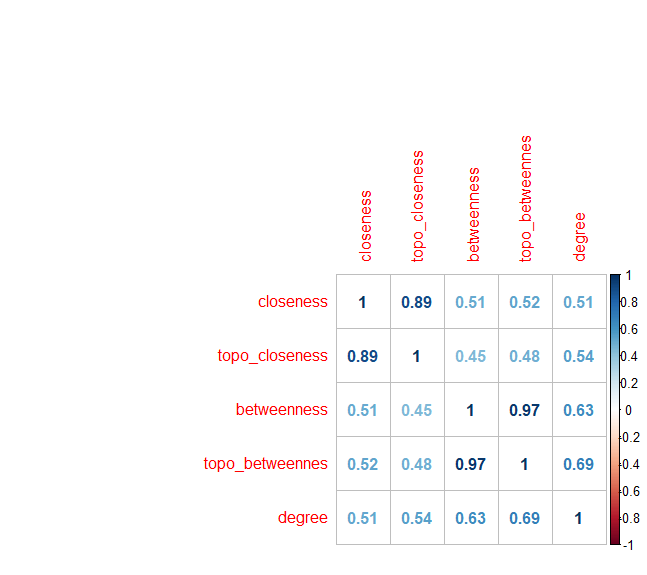
\includegraphics[width=0.8\textwidth]{example}
\caption{Correlation between station/node metrics}
\end{figure}

\begin{tabular}{|l|l|l|l|}\hline
  \multirow{10}{*}{numeric literals} 				& \multirow{5}{*}{integers} 	& in decimal 					& \verb|8743| \\ \cline{3-4}
  					    				& 				       	& \multirow{2}{*}{in octal}   		& \verb|0o7464| \\ \cline{4-4}
  					    				& 					& 						& \verb|0O103| \\ \cline{3-4}
  					    				& 					& \multirow{2}{*}{in hexadecimal}	& \verb|0x5A0FF| \\ \cline{4-4}
 				 	    				& 					& 						& \verb|0xE0F2| \\ \cline{2-4}
  					    				& \multirow{5}{*}{fractionals} 	& \multirow{5}{*}{in decimal} 		& \verb|140.58| \\ \cline{4-4}
 				 					& 					& 						& \verb|8.04e7| \\ \cline{4-4}
  									& 					& 						& \verb|0.347E+12| \\ \cline{4-4}
  									& 					& 						& \verb|5.47E-12| \\ \cline{4-4}
  									& 					& 						& \verb|47e22| \\ \cline{1-4}
  \multicolumn{3}{|l|}{\multirow{3}{*}{char literals}} 													& \verb|'H'| \\ \cline{4-4}
  \multicolumn{3}{|l|}{} 																	& \verb|'\n'| \\ \cline{4-4}          %% here
  \multicolumn{3}{|l|}{} 																	& \verb|'\x65'| \\ \cline{1-4}        %% here
  \multicolumn{3}{|l|}{\multirow{2}{*}{string literals}} 												& \verb|"bom dia"| \\ \cline{4-4}
  \multicolumn{3}{|l|}{} 																	& \verb|"ouro preto\nmg"| \\ \cline{1-4}          %% here
\end{tabular}




\begin{verbatim}
use pseudocode
\end{verbatim}

\textit{italics}
\textbf{bold}

XXXX words excluding headings, figures, and references. \\

\nocite{*}

\medskip


\printbibliography


\end{document}
